\section{Terapie}
Sono numerose le malattie che possono danneggiare i reni ed alcune di queste portano inesorabilmente alla perdita della loro funzionalità. Quando questo avviene le uniche possibilità terapeutiche per il paziente sono il trapianto di rene e la dialisi.

\subsection{Trapianto \cite{hsr}}
L'intervento chirurgico di trapianto prevede l'anastomosi dei vasi del rene con i vasi iliaci del ricevente, e l'attacco del'uretere, proveniente dallo stesso donatore, alla vescica. Come è necessario nel caso di tutti i trapianti di organo o tessuto, anche nel caso del trapianto di rene devono essere somministrati farmaci immunosoppressori per evitarne il rigetto.
Il trapianto può essere eseguito prelevando l'organo da cadavere o da un donatore vivente. Il vantaggio del trapianto di rene da donatore vivente è legato alla sua programmabilità e ad una probabilità di successo superiore al trapianto da cadavere.  L'individuo che volontariamente si offre ad una donazione di rene esegue una serie di accertamenti che mirano ad escludere la possibilità che egli stesso abbia una nefropatia latente o una patologia che ne favorisca lo sviluppo in futuro. L'atto chirurgico del prelievo del rene può essere eseguito per via laparoscopica e quindi con ridotta invasività.

\subsection{Dialisi}\label{sub:dialisi}
Col termine \textit{dialisi} ci si riferisce a un processo di purificazione di un fluido per mezzo di un'altro fluido, detto dializzante, separato dal primo attraverso una membrana semipermeabile, artificiale o biologica. A seconda della tecnica di dialisi, gli scambi di massa attraverso la membrana avvengono per diffusione e/o convezione.

\subsubsection{Dialisi peritoneale}
\begin{wrapfigure}{O}{0.32\textwidth}
	\centering
		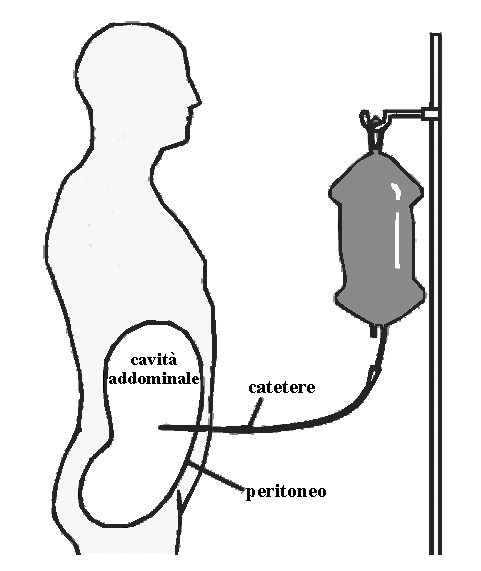
\includegraphics[width=0.32\textwidth]{immagini/peritoneale.eps}
		\vspace{-20pt}
		\caption{}\label{peritoneale}
		\vspace{-10pt}
\end{wrapfigure}
La dialisi peritoneale sfrutta come membrana semipermeabile il peritoneo, che è la membrana che costituisce il rivestimento della cavità addominale (\figurename~\ref{peritoneale}). Attraverso un catetere trans-dermico si riempie l'addome col liquido dializzante, permettendo così uno scambio diffusivo di soluti fra i vasi del peritoneo e il fluido dializzante. È anche possibile, oltre ai cataboliti, estrarre fluidi corporei in eccesso (ultrafiltrazione) giocando sull'osmolarità del liquido dializzante. Il dialisato è mantenuto nella cavità addominale per il tempo necessario agli scambi. Il ciclo è ripetuto fino a dieci volte al giorno, talvolta con l'ausilio notturno di un dispositivo automatico per il riempimento e svuotamento dell'addome \cite{casagrande}. Questa tecnica \textit{auto-terapica} richiede molta diligenza da parte del paziente, ma facendo uso di dispositivi semplici e poco ingombranti, rende il soggetto in dialisi (quasi) indipendente dai centri specializzati.
 
\subsubsection{Emodialisi}
L'emodialisi (HD) è una terapia che permette di purificare il sangue del paziente tramite un filtro detto \textit{dializzatore}, ovvero rene artificiale. Diversamente dal rene biologico che è in grado anche di riassorbire attivamente sostanze utili dal filtrato glomerulare, il rene artificiale esercita sulla composizione del plasma un ruolo puramente passivo. L'eliminazione delle sostanze di scarto (urea, creatinina ed altre) avviene semplicemente ponendo a contatto, tramite la membrana del dializzatore, il sangue da filtrare con una soluzione dializzante di composizione simile a quella che fisiologicamente dobrebbe avere il plasma.

\begin{wrapfigure}{O}{0.32\textwidth}
	\centering
	\vspace{-30pt}
		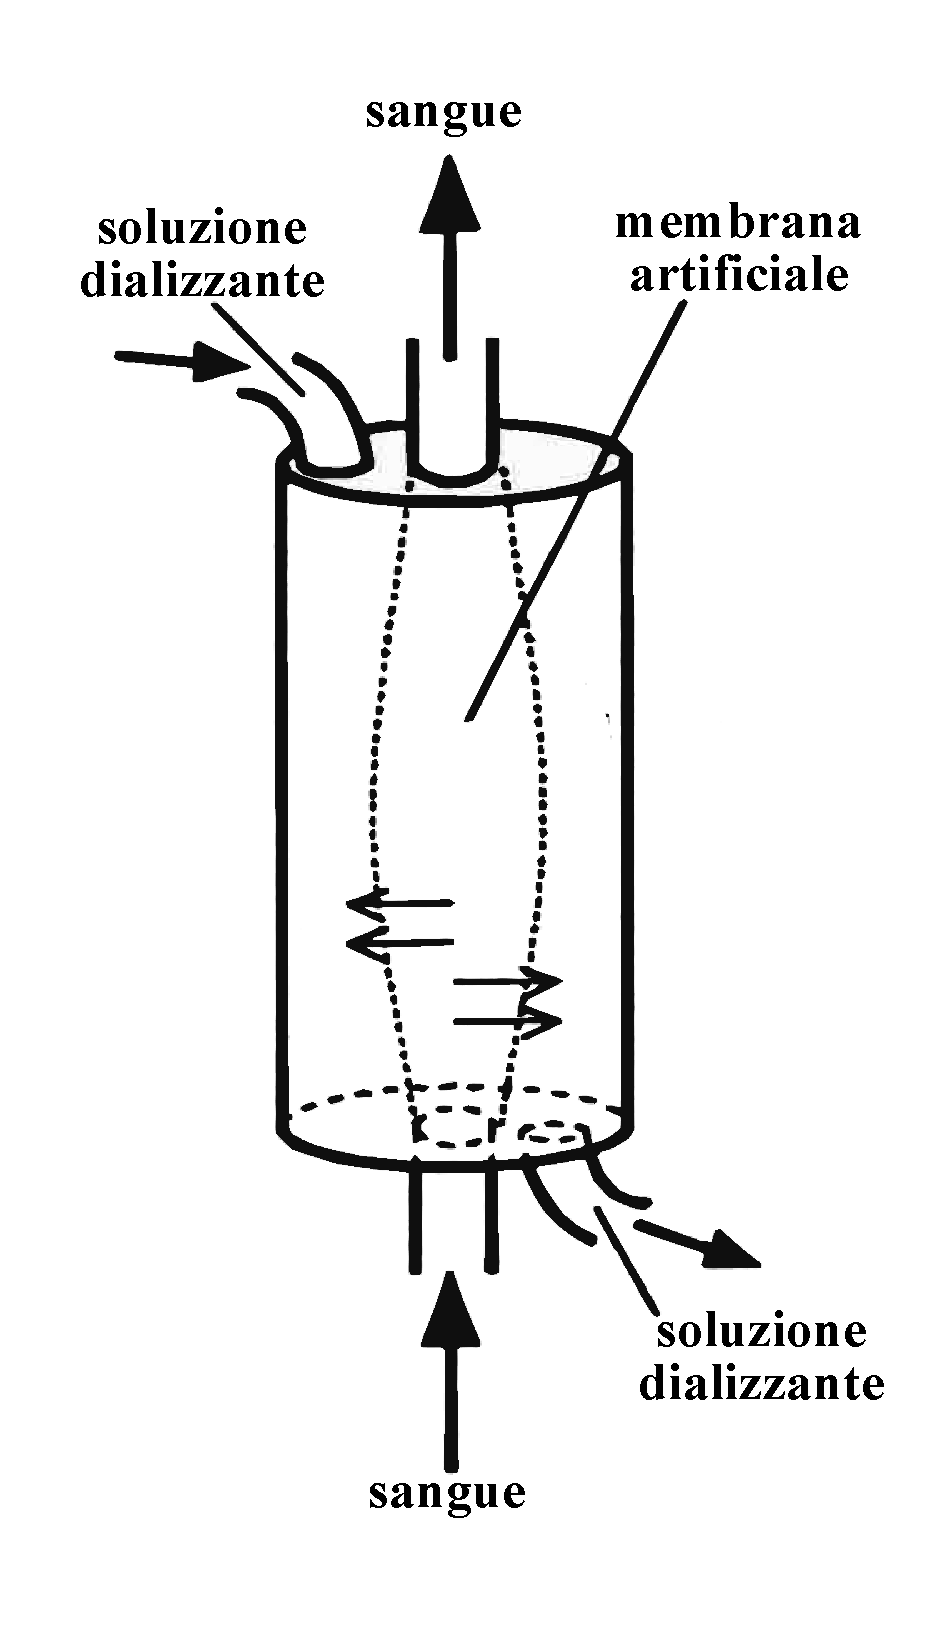
\includegraphics[width=0.32\textwidth]{immagini/emod.eps}
		\vspace{-30pt}
		\caption{}\label{membHD}
		\vspace{-10pt}
\end{wrapfigure}

Il dializzatore, rudemente schematizzato in \figurename~\ref{membHD}, è costituito da una membrana semipermeabile artificiale che trattiene i globuli rossi e le proteine del plasma e permette la diffusione delle molecole di scarto, a basso peso molecolare, dal plasma al liquido dializzante. La concentrazione dei soluti nel plasma, elevata all'inizio della seduta, diminuisce nel corso della dialisi fino a raggiungere, in teoria, la stessa concentrazione del dialisato. Inoltre, per permettere l'eliminazione dei fluidi accumulati durante il periodo interdialitico, è necessario mantenere una modesta differenza di pressione idraulica tra il compartimento ematico e quello del dialisato, in modo che parte del solvente (acqua) dal sangue attraversi la membrana e venga eliminata. Al processo di diffusione allora si aggiunge quindi anche quello di convezione. La quantità di acqua così eliminata, circa mezzo litro l'ora, deve essere controllata nel corso della dialisi insieme alle condizioni generali del paziente, poiché una brusca e notevole diminuzione del volume plasmatico può portare al collasso cardio-circolatorio.

\subsubsection{Emofiltrazione}
L'emofiltrazione (HF) è una tecnica dialitica in cui la rimozione di soluti avviene quasi esclusivamente per convezione. Per l'alta porosità delle membrane qui usate, se si applica un'adeguata pressione di trans-membrana è possibile rimuovere un elevato volume di acqua, dell'ordine della decina di litri a seduta, la quale trasporta con sè le sostanze in essa disciolte; poiché una perdita così elevata di fluidi non è sostenibile dall'organismo umano, è necessario reinfondere la maggior parte del volume filtrato con un adeguato flusso di liquido di sostituzione, ovvero di diluizione, a monte o a valle rispetto al dializzatore, cioè in pre- o post-diluizione. La porosità della membrana è un parametro importante nel trasporto per convezione, perché rende possibile la rimozione prodotti di scarto di peso molecolare medio/alto, cosa che con non è possibile con le normali membrane per emodialisi.

\subsubsection{Emodiafiltrazione}
Il termine \textit{emodiafiltrazione} (HDF) fu utilizzato per la prima volta da Leber et al. \cite{leber} in Germania e fu proposto come un nuovo metodo per la purificazione del sangue ottenuta tramite la combinazione equilibrata di diffusione e convezione.
L'HDF può difatti essere definita come una tecnica di dialisi che utilizza membrane altamente permeabili, nelle quali la diffusione e la convezione sono equamente determinanti per la rimozione di soluti/tossine di vario peso molecolare.
Uno dei grandi risultati dell'HDF è infatti quello di poter rimuovere non solo soluti a basso peso molecolare, come accade per l'emodialisi, ma anche molecole ritenute dannose, come le $\beta_2$-microglobuline ($11,8$ $kDa$), che fanno parte della categoria delle sostanze a medio/alto peso molecolare.
Inizialmente nella dialisi erano i soli processi diffusivi a regolare la purificazione del sangue e ciò a causa della bassa permeabilità idraulica delle membrane e della porosità insufficiente a permettere alti flussi. Grazie allo sviluppo di polimeri sintetici, con una struttura ibrida idrofilica e idrofobica e uno spessore di membrana ridotto, si è potuto sfruttare anche il processo convettivo di purificazione ematica e dare quindi il via alla tecnica dell'emodiafiltrazione.
Nell'HDF  il trasporto di soluti può avvenire e per diffusione e per convezione. Il trasporto diffusivo è descritto dalla legge di Fick, espressa matematicamente da $$J_d = -D_s \frac{dC_s}{dx}$$
dove $J_d$ è il flusso netto diffusivo, $D_s$ il coefficiente di diffusione del soluto in esame e $C_s$ la sua concentrazione.
Il trasporto convettivo è invece caratterizzato dalla filtrazione di fluido attraverso la membrana come conseguenza di un gradiente locale di pressione; in formule:
$$J_c = L_p \biggl(\Delta P - \Delta\Pi\biggr)C_M$$
dove $L_p$ è la permeabilità idraulica della membrana, $\Delta P$ il gradiente idraulico e $\Delta \Pi$ il gradiente osmotico a cavallo della membrana e  $C_M$ la concentrazione di membrana media del soluto trasportato.
L'efficienza dell'HDF è influenzata, come per l'emodialisi, dalla portata di sangue prelevato dalla fistola o dal catetere venoso, dalla portata del dialisato, dall'ematocrito e dal proteinocrito (dall'inglese \textit{protocrit}, cioè la frazione di proteine nel plasma). L'efficienza dipende anche dalla modalità di infusione del fluido di sostituzione (pre-diluizione o post-diluizione). A parità di altre condizioni, in post-diluizione la \textit{clearance} delle molecole a basso/medio peso molecolare è maggiore rispetto all'emodialisi. Il sangue però rischia di coagulare all'interno del dializzatore a seguito dell'emoconcentrazione che avviene lungo i capillari. In pre-diluizione invece il sangue ha proprietà reologiche meno favorevoli alla coagulazione ma, a causa della diluizione, la cleareance dei soluti risulta diminuita \cite{hoenich}.

\subsubsection{Tipologie di HDF}
L'emodiafiltrazione è una combinazione di emodialisi e emofiltrazione che rende possibile la rimozione simultanea e ottimale di soluti a basso e alto peso molecolare. Il contributo relativo della convezione rispetto alla diffusione, aumenta all'aumentare del peso molecolare del soluto da rimuovere. Questi concetti sono stati applicati nella pratica clinica portando allo sviluppo di diverse tipologie di HDF, descritte da C.~Ronco \cite{evolutionHDF}, che illustreremo nei prossimi paragrafi.

\paragraph{HDF classica.}
\begin{wrapfigure}{o}{0.35\textwidth}
	\centering
	\vspace{-10pt}
		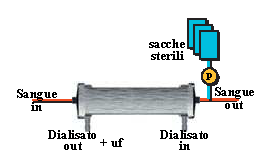
\includegraphics[width=0.35\textwidth]{immagini/classicHDF.eps}
		\vspace{-20pt}
\end{wrapfigure}
Questa tipologia di trattamento è caratterizzata da portate di reinfusione di circa $3$-$15$~$L$ a seduta, tipicamente in post-diluizione. Il liquido di diluizione è contenuto in apposite sacche sterili. Per ottenere regimi di ultrafiltrazione pressori di trans-membra accettabili, sono necessarie portate ematiche superiori ai $300$~$mL/min$. Questa tecnica è stata utilizzata per molti anni fino a quando non sono state disponibili modalità più economiche di produzione del fluido di diluizione (cfr. \textit{on-line} HDF).

\paragraph{On-line HDF.}
\begin{wrapfigure}{o}{0.40\textwidth}
	\centering
	\vspace{-10pt}
		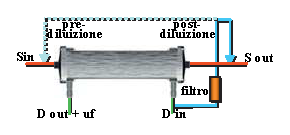
\includegraphics[width=0.40\textwidth]{immagini/onlineHDF.eps}
		\vspace{-20pt}
\end{wrapfigure}
La necessità di alternative per l'elevato costo delle sacche di reinfusione, e il miglioramento delle tecnologie per la preparazione del liquido di dialisi, hanno permesso lo sviluppo di una nuova tecnica chiamata \textit{on-line} HDF. In questa modalità, del dialisato ultrapuro è preparato al momento dell'uso dalla macchina dializzatrice. La qualità del fluido prodotto è eccellente, ed è garantita dalla ridondanza dei sistemi di filtraggio. Attraverso celle conduttimetriche e pompe, la macchina regola automaticamente la diluizione delle soluzioni concentrate, per ottenere i valori giusti di concentrazione impostati per lo specifico paziente. Questo procedura rende disponibile immediatamente e a basso costo una grande quantità di liquido di sostituzione e l'HDF può essere portata a termine con un elevato ricambio di fluido (intorno ai $40$~$L/sessione$) utilizzando la pre- o la post-diluizione o, ancora in fase sperimentale \cite{pedrini}, un mix delle due modalità.

\paragraph{Internal-Filtration HDF.}
Quando un dializzatore ad alta permeabilità è usato in condizioni di minima ultrafiltrazione si può erroneamente pensare che il processo di scambio avvenga per sola diffusione. Gli scambi convettivi, mascherati invece dalla cinetica interna della \textit{retro-filtrazione}, non sono affatto trascurabili. Il fenomeno è del tutto paragonabile a ciò che avviene nel letto capillare umano secondo l'ipotesi di Starling (\figurename~\ref{starling}): man mano che si avanza nel lato sangue lungo i capillari del dializzatore, la pressione idraulica diminuisce fino al punto in cui è possibile che la pressione di trans-membrana si inverta, richiamando liquido dializzante nel lume ematico. Questo fenomeno può essere amplificato applicando, per esempio, una restrizione verso la metà del fascio di capillari, oppure riducendo il diametro interno delle fibre. In questo modo la retro-filtrazione può raggiungere valori di $40$-$50$ $mL/min$ con un dializzatore da $1.8$~$m^2$ in regime di ultrafiltrazione netta nulla. Anche se questo fenomeno avviene in qualsiasi dializzatore ad alta permeabilità, quando specifici accorgimenti e particolari design sono usati per favorire la retro-filtrazione, la tecnica dialitica prende il nome di internal-HDF.

\paragraph{Paired Filtration.}
\begin{wrapfigure}{o}{0.35\textwidth}
	\centering
	\vspace{-10pt}
		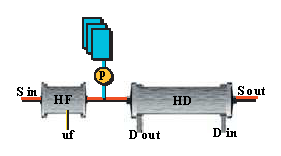
\includegraphics[width=0.35\textwidth]{immagini/paired.eps}
		\vspace{-15pt}
\end{wrapfigure}
Questa tipologia di HDF è stata concepita per la prima volta in Italia. È caratterizzata da due dializzatori posti in serie: il primo è molto poroso e la convezione è dominante, il secondo è un classico emodializzatore nel quale è la diffusione il fenomeno dominante. Il fluido di diluizione è immesso nel circuito tra un filtro e l'altro. Lo scopo di questo design è quello di minimizzare le interazioni sfavorevoli tra convezione e diffusione, di prevenire la retro-filtrazione e di ottenere misure più accurate sull'ultrafiltrato essendo questo provvisto di una linea separata dalla linea di uscita del dialisato.

\paragraph{Mid-diluition HDF.}
\begin{wrapfigure}{o}{0.35\textwidth}
	\centering
	\vspace{-10pt}
		
\includegraphics[width=0.35\textwidth]{immagini/midHDF.eps}
		\vspace{-20pt}
\end{wrapfigure}
Per questo tipo di HDF è necessario un filtro particolare costituito da due compartimenti longitudinali posti idraulicamente in serie. Il sangue entra nel primo compartimento in contro-corrente al dialisato; qui avviene l'ultrafiltrazione. Quando il sangue, emoconcentrato, giunge alla fine del primo compartimento viene diluito col fluido di sostituzione e immesso nel secondo compartimento, iso-corrente al dialisato. Il sangue in uscita lascia il dializzatore da una porta vicina a quella di ingresso.

\paragraph{Double High-Flux HDF.}
\begin{wrapfigure}{o}{0.40\textwidth}
	\centering
	\vspace{-10pt}
		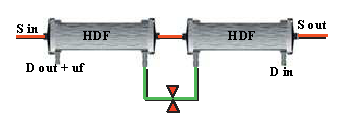
\includegraphics[width=0.40\textwidth]{immagini/doubleHDF.eps}
		\vspace{-20pt}
\end{wrapfigure}
Si utilizzano due dializzatori ad alta porosità posti in serie. La filtrazione avviene nell'unità prossimale e la retro-filtrazione in quella distale. La retro-filtrazione, ovvero la portata del fluido di diluizione, può essere modulata da una resistenza idraulica posta sulla linea del dialisato congiungente i dializzatori. Quando si riescono a raggiungere alti flussi di fistola ($>500$~$mL/min$) l'alta efficienza di questa metodologia permette trattamenti della durata inferiore alle due ore \cite{miller}.


\paragraph{Push-Pull HDF.}
\begin{wrapfigure}{o}{0.40\textwidth}
	\centering
		
\includegraphics[width=0.40\textwidth]{immagini/pushpull.eps}
		\vspace{-20pt}
\end{wrapfigure}
Con questa tecnica è possibile variare il rapporto fra filtrazione e retro-filtrazione. La rotazione della pompa pre-filtro (mentre quella post-filtro è ferma) produce filtrazione; la rotazione della pompa post-filtro (mentre è ferma quella pre-filtro) genera una pressione negativa nel compartimento ematico e quindi retro-filtrazione. Le pompe di modulazione possono in alternativa essere poste sulla linea del dialisato.

\section{Conclusioni}
In questo capitolo sono state descritte le problematiche che una patologia renale comporta e, molto sinteticamente, le varie terapie dialitiche usate in ambito clinico per depurare l'organismo a seguito di tale patologia. Nel prossimo capitolo si descriverà in maniera più approfondita la tecnica oggetto di modellizzazione in questa tesi: l'\textit{on-line} HDF.